\documentclass[10pt,a4paper]{article}% ===> this file was generated automatically by noweave --- better not edit it
\usepackage[margin=25mm]{geometry}
\usepackage{pgf,tikz}
\usepackage{subfig}
\usepackage{amsmath}
\usepackage{amssymb}
\usepackage{noweb}
\usepackage{amsthm}
\usepackage{hyperref}
\setlength{\parskip}{3mm}
\newtheorem{axiom}{Axiom}
\newtheorem{definition}{Definition}
\newtheorem{comment}{Comment}
\newtheorem{example}{Example}
\newtheorem{lemma}{Lemma}
\newtheorem{prop}{Property}
\newtheorem{remark}{Remark}
\newtheorem{theorem}{Theorem}
\author{Dilawar Singh \\
Email : \texttt{dilawar@ee.iitb.ac.in}}
\title{Flow Network Using {\Tt{}Graph-tool\nwendquote}}
\begin{document}
\nwfilename{flow_in_graphs.snw}\nwbegindocs{1}\nwdocspar
\maketitle
\begin{abstract}
    
    In this document, we solve some simple networks for max-flow using
    {\Tt{}graph-tool\nwendquote} - a python bindings for famous boost graph libraries. This
    package is very useful for rapid prototyping. \footnote{Add a note on their
    performance with respect to boost graph libraries}.

\end{abstract}

\nwenddocs{}\nwbegindocs{2}\section{First thing first}

Here is overall code-structure of this excercise.

\nwenddocs{}\nwbegincode{3}\moddef{*}\endmoddef\nwstartdeflinemarkup\nwenddeflinemarkup
\LA{}Import\RA{}
\LA{}Initialise\RA{}
\LA{}Subroutines\RA{}
\LA{}Test cases\RA{}
\LA{}Create flow network\RA{}
\LA{}Calculate flow on network\RA{}
\LA{}Save the work for posterity\RA{}
#ipshell()
\eatline
\nwendcode{}\nwbegindocs{4}\nwdocspar

@\paragraph{Import {\Tt{}graphs-tool\nwendquote} and others}. 
    
    It is a wrapper written on boost-graph libraries written for python. It
    allows one to do rapid prototyping. When an idea is tested, one can rewrite
    the whole thing in C++ when performance really matters.

    We surely need to import it. Make sure you have it installed. It is freely
    available. And I like issuing warning!

\nwenddocs{}\nwbegincode{5}\moddef{Import}\endmoddef\nwstartdeflinemarkup\nwenddeflinemarkup
from graph_tool.all import * 
import warnings as warn
\nwendcode{}\nwbegindocs{6}And we also need {\Tt{}Ipython\nwendquote} for better interaction with Hobbes \footnote{My
personal computer}.

    Python interpretor is not very user-friendly (there is not 'tab'
    completion). This has been changed in hugely improved {\Tt{}ipython\nwendquote} shell. Why
    not use it!

\nwenddocs{}\nwbegincode{7}\moddef{Import}\plusendmoddef\nwstartdeflinemarkup\nwenddeflinemarkup
try:
    __IPYTHON__
except NameError:
    from IPython.Shell import IPShellEmbed
    ipshell = IPShellEmbed()
    # Now ipshell() will open IPython anywhere in the code
else:
    # Define a dummy ipshell() so the same code doesn't crash inside an
    # interactive IPython
    def ipshell(): pass

\nwendcode{}\nwbegindocs{8}And now we are ready to initialize a graph, we'll use this particular graph
much later though.

\nwenddocs{}\nwbegincode{9}\moddef{Initialise}\endmoddef\nwstartdeflinemarkup\nwenddeflinemarkup
g = Graph()

\nwendcode{}\nwbegindocs{10}\section{A small example to test the platform}

    A flow network is a directed graph $G(V,E,s,t)$ where $V\cup \{s,t\}$ are
    vertices and $E$ are set of edges, $s$ is source node and $t$ is sink node.
    A source node does not have any incoming edge while a sink node does not
    have any outgoing edge.

    Now, we need to define property maps on nodes and edges.

    To solve a graph problem, we first attach some properties to the edges and
    nodes of graph such as distance, capacity, weight, color etc. 

    Each node in a flow graph $G$ has an index: 0 and 1 index is always reserved
    for Source/sink nodes.  An optional {\Tt{}name\nwendquote} can also be attached to the
    graph nodes. 

    An edge in $G$ is more complicated. It has a maximum flow capacity
    {\Tt{}capcity\nwendquote} (integer), flow value {\Tt{}flow\nwendquote} (integer) and a name {\Tt{}tag\nwendquote}.

    Lpet's create a trivial flow network and add some vertices to this graph.

\nwenddocs{}\nwbegincode{11}\moddef{Initialise}\plusendmoddef\nwstartdeflinemarkup\nwenddeflinemarkup
g = Graph()

\nwendcode{}\nwbegindocs{12}  On this graph {\Tt{}g\nwendquote}, lets define properties which we can assign to edges
    and nodes. For example, we'd like to give names to edges and nodes (although
    index is sufficient to distinguish vertices and edges). More importantly, we
    have to give capacity to each edge and we'd like to store computed flow in
    some property map. I may be using too much of fore-sight. Not all of these
    properties will be used. What the heck, more is good!

\nwenddocs{}\nwbegincode{13}\moddef{Properties on edges and nodes}\endmoddef\nwstartdeflinemarkup\nwenddeflinemarkup
v_name = g.new_vertex_property("string") # name of vertex
e_name = g.new_edge_property("string") # name of edge 
e_caps = g.new_edge_property("int32_t") # capacity on edges (must)
e_flow = g.new_edge_property("int32_t") # flow (optional)


\nwendcode{}\nwbegindocs{14}  It is always useful to create a figure of what you are doing. It uses
    {\Tt{}dot\nwendquote} tool to draw the graphs by passing properties such as position of
    nodes, vertex color, edges type etc. You better look at the documentation of
    dot and graph-tool for futher details. Anyway, we show one property -
    position of nodes
    - which can be passed to {\Tt{}dot\nwendquote}.

\nwenddocs{}\nwbegincode{15}\moddef{Properties on edges and nodes}\plusendmoddef\nwstartdeflinemarkup\nwenddeflinemarkup
v_pos = g.new_vertex_property("vector<double>")

\nwendcode{}\nwbegindocs{16}Now we are ready to create flow network.
\nwenddocs{}\nwbegincode{17}\moddef{Create flow network}\endmoddef\nwstartdeflinemarkup\nwenddeflinemarkup
\LA{}Properties on edges and nodes\RA{}

\nwendcode{}\nwbegindocs{18}  What about fixing the position of nodes. Let's assume that I want all
    nodes in a line separated by 2 units. Following is my network which I want
    to solve. It's trivial so that one can verify the solution returned by
    {\Tt{}graph-tool\nwendquote}.

\begin{figure}[h]
\centering
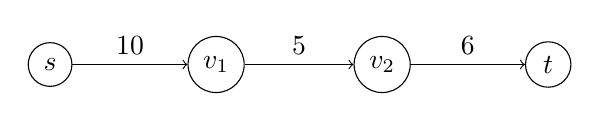
\begin{tikzpicture}[x=30,y=30]
\node[circle, draw] (s) at (0,0) {$s$};
\node[circle, draw] (v1) at (2,0) {$v_1$};
\node[circle, draw] (v2) at (4,0) {$v_2$};
\node[circle, draw] (t) at (6,0) {$t$};
\path[->] (s) edge  node[above, sloped] {$10$} (v1)
          (v1) edge  node[above, sloped, midway] {$5$} (v2)
          (v2) edge  node[above, sloped, midway] {$6$} (t)
          ;
\end{tikzpicture}
\caption{\small A flow path}
\label{fig:flow_path}
\end{figure}

\nwenddocs{}\nwbegincode{19}\moddef{Create flow network}\plusendmoddef\nwstartdeflinemarkup\nwenddeflinemarkup
g.add_vertex(4) # a flow path with 4 vertex.
i = 0.0
for v in g.vertices():
    v_pos[g.vertex(v)] = [i,0.0]
    i += 2.0 # gap of 2 units
# we need to fix 0 and 1 manually
v_pos[g.vertex(0)] = [0.0,0.0]
v_pos[g.vertex(1)] = [6.0,0.0]


\nwendcode{}\nwbegindocs{20}  Now we add some edge to our trivial network. Out trivial network is going
    to be a simple path. Now we put these capacity values in property map
    {\Tt{}e{\_}caps\nwendquote}.

\nwenddocs{}\nwbegincode{21}\moddef{Create flow network}\plusendmoddef\nwstartdeflinemarkup\nwenddeflinemarkup
e12 = g.add_edge(g.vertex(0), g.vertex(2))
e_caps[e12] = 10
e23 = g.add_edge(g.vertex(2), g.vertex(3))
e_caps[e23] = 5
e31 = g.add_edge(g.vertex(3), g.vertex(1))
e_caps[e31] = 6

\nwendcode{}\nwbegindocs{22}\begin{remark} 
    
    These properties on vertex or edges are not the property of
    graph as such. It is useful to make them property of graph so that when we
    save this graph to a file, we save these properties too. Then we can simply
    load the graph and Hey Presto, we don't have to put values in property map.
    \footnote{Please look at the boost library documentation on property maps}.
    
\end{remark}

\nwenddocs{}\nwbegincode{23}\moddef{Convert to graph properties}\endmoddef\nwstartdeflinemarkup\nwenddeflinemarkup
g.edge_properties["cap"] = e_caps 

\nwendcode{}\nwbegindocs{24}Now we should save this work. We may like to use this graph again some day.
Also let's make a figure for our graph.

\nwenddocs{}\nwbegincode{25}\moddef{Save the work for posterity}\endmoddef\nwstartdeflinemarkup\nwenddeflinemarkup
\LA{}Convert to graph properties\RA{}
g.save("graphs/simple_flow_path.xml.gz")
# and print also.
graph_draw(g , pos=v_pos
    , vprops=\{"label":g.vertex_index\}
    , eprops = \{"label":e_caps\}
    , output="figs/simple_flow.pdf")

\nwendcode{}\nwbegindocs{26}Lets see, how {\Tt{}dot\nwendquote} has drawn our figure.
\begin{figure}[h]
\centering
\includegraphics[width=0.75\textwidth]{figs/simple_flow.pdf}
\caption{Flow path drawn by graph-tool. We are using index (integer) rather than
ame to distinguish the vertices. Also index 0 and 1 are source and sink vertex.
Compare it with previous fig \ref{fig:flow_path}. {\Tt{}dot\nwendquote} has inbuilt algorithms
to handle very large graph. See documentation for more details.}
\end{figure}

\nwenddocs{}\nwbegindocs{27}Now, it's time to solve this network. This package {\Tt{}graph-tool\nwendquote} gives 3
    well known algorithms: {\Tt{}edmond{\_}karp{\_}max{\_}flow\nwendquote}, {\Tt{}push{\_}relable{\_}max{\_}flow\nwendquote},
    and {\Tt{}boykov{\_}kolmogorov{\_}max{\_}flow\nwendquote}. Lets write some functions to automate
    this task.

\nwenddocs{}\nwbegincode{28}\moddef{Subroutines}\endmoddef\nwstartdeflinemarkup\nwenddeflinemarkup
def edmondKarp(graph, prop):
    src, tgt = graph.vertex(0), graph.vertex(1)
    res = edmonds_karp_max_flow(graph, src, tgt, prop) # graph-tool method
    res.a = prop.a - res.a
    max_flow = sum(res[e] for e in tgt.in_edges())
    return max_flow, res.a
\eatline
\nwendcode{}\nwbegindocs{29}\nwdocspar
\nwenddocs{}\nwbegincode{30}\moddef{Subroutines}\plusendmoddef\nwstartdeflinemarkup\nwenddeflinemarkup
def pushRelabel(graph, prop):
    src, tgt = graph.vertex(0), graph.vertex(1)
    res = push_relabel_max_flow(graph, src, tgt, prop)
    res.a = prop.a - res.a
    max_flow = sum(res[e] for e in tgt.in_edges())
    return max_flow, res.a
\eatline
\nwendcode{}\nwbegindocs{31}\nwdocspar
\nwenddocs{}\nwbegincode{32}\moddef{Subroutines}\plusendmoddef\nwstartdeflinemarkup\nwenddeflinemarkup
def kolmogorov(graph, prop):
    src, tgt = graph.vertex(0), graph.vertex(1)
    res = boykov_kolmogorov_max_flow(graph, src, tgt, prop)
    # here we have a bug. res returned by above method does not have the same length
    # as others.
    if res.a.size == prop.a.size:
         res.a = prop.a - res.a
    else:
        warn.warn("Loop found here. This method can't handle it")
        return -1, res.a
    max_flow = sum(res[e] for e in src.out_edges())
    return max_flow, res.a
\nwendcode{}\nwbegindocs{33}\nwdocspar
\nwenddocs{}\nwbegincode{34}\moddef{Calculate flow on network}\endmoddef\nwstartdeflinemarkup\nwenddeflinemarkup
max_flow1, res1 = edmondKarp(g, e_caps)
max_flow2, res2 = pushRelabel(g, e_caps)
max_flow3, res3 = kolmogorov(g, e_caps)
print max_flow1, max_flow2, max_flow3

\nwendcode{}\nwbegindocs{35}\section{Testing} 
 
    Now it is a good time, to inlcude some testing
    frameworks. Pyhton provides a good testing module {\Tt{}unittest\nwendquote}. Lets import
    it.

\nwenddocs{}\nwbegincode{36}\moddef{Import}\plusendmoddef\nwstartdeflinemarkup\nwenddeflinemarkup
import unittest

\nwendcode{}\nwbegindocs{37}Now, we create a class with will all out tests. We can add new
    properties as we go along on our journey.

\nwenddocs{}\nwbegincode{38}\moddef{Test cases}\endmoddef\nwstartdeflinemarkup\nwenddeflinemarkup
class GraphTestClass(unittest.TestCase):  
    # this is responsible in setting up the test-bench.
    def setUp(self): pass

    def createData(self, g, prop):
        self.flow1, self.res1 = edmondKarp(g, prop)
        self.flow2, self.res2 = pushRelabel(g, prop)
        self.flow3, self.res3 = kolmogorov(g, prop)
 
class TestForEquality(GraphTestClass):
    # add tests here.
    \LA{}Add tests\RA{}

\eatline
\nwendcode{}\nwbegindocs{39}\nwdocspar
    @ Before we proceed, it's not a bad idea to define some trivial properties.
    For example, check if all three available algorithms are producing same
    answers.

\nwenddocs{}\nwbegincode{40}\moddef{Add tests}\endmoddef\nwstartdeflinemarkup\nwenddeflinemarkup
# for graph g1
def testEqualG1(self):
    self.createData(g, e_caps)
    if self.flow1 > 0 and self.flow2 > 0 and self.flow3 > 0 : 
        self.assertEqual(self.flow1, self.flow2)
        self.assertEqual(self.flow2, self.flow3)
        self.assertEqual(self.res1.all(), self.res2.all())
        self.assertEqual(self.res2.all(), self.res3.all())
    else:
        warn.warn("Negative Flow. One of more method is unsuitable.")

\nwendcode{}\nwbegindocs{41}And the anwer is 5 and it passes the test i.e. all algorithms are producing
equal values.

\nwenddocs{}\nwbegindocs{42}\section{Another example}

    So far, so good! Now lets make things more complicated. We'll solve a well
    known given in a book \textbf{Introduction to Algorithms} on page 659 and
    see if our results matches with theirs. Following figure shows this
    particular example.

\begin{figure}[h]
\centering
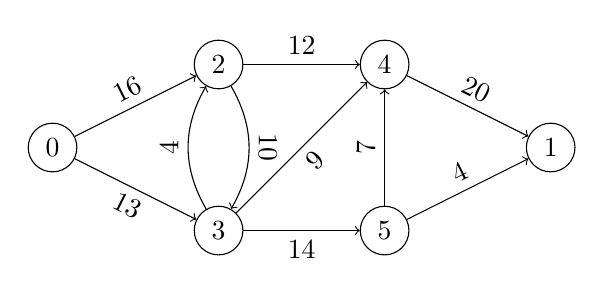
\begin{tikzpicture}[x=30,y=30]
\node[circle, draw] (s) at (0,0) {$0$};
\node[circle, draw] (v1) at (2,1) {$2$};
\node[circle, draw] (v2) at (2,-1) {$3$};
\node[circle, draw] (v3) at (4,1) {$4$};
\node[circle, draw] (v4) at (4,-1) {$5$};
\node[circle, draw] (t) at (6,0) {$1$};
\path[->] (s) edge node[above, sloped] {$16$} (v1)
              edge node[below, sloped] {$13$} (v2)
          (v1) edge[bend left] node[above, sloped, midway] {$10$} (v2)
               edge node[above, sloped] {$12$} (v3)
          (v2) edge[bend left]  node[above, sloped, midway] {$4$} (v1)
               edge node [sloped, below] {$9$} (v3)
               edge node [below] {$14$} (v4)
          (v3) edge node [sloped, above] {$20$} (t)
          (v4) edge node [sloped, above] {$7$} (v3)
          (v4) edge node [sloped, above] {$4$} (t)
          ;
\end{tikzpicture}
\caption{\small A flow network}
\label{fig:flow_network}
\end{figure}

\nwenddocs{}\nwbegindocs{43}Let's call this graph $g1$ and add edges and vertices to it.

\nwenddocs{}\nwbegincode{44}\moddef{Initialise}\plusendmoddef\nwstartdeflinemarkup\nwenddeflinemarkup
g1 = Graph()

\nwendcode{}\nwbegincode{45}\moddef{Properties on edges and nodes}\plusendmoddef\nwstartdeflinemarkup\nwenddeflinemarkup
vName = g1.new_vertex_property("string")
eName = g1.new_edge_property("string")
eCaps = g1.new_edge_property("int32_t")
eFlow = g1.new_edge_property("int32_t")
\nwendcode{}\nwbegindocs{46}\nwdocspar


\nwenddocs{}\nwbegincode{47}\moddef{Create flow network}\plusendmoddef\nwstartdeflinemarkup\nwenddeflinemarkup
# total 6 vertices. O and 1 are source and sink vertex.
g1.add_vertex(6)

# add edges and assigned capacity.
e02 = g1.add_edge(g1.vertex(0), g1.vertex(2))
eCaps[e02] = 16
e03 = g1.add_edge(g1.vertex(0), g1.vertex(3))
eCaps[e03] = 13

e24 = g1.add_edge(g1.vertex(2), g1.vertex(4))
eCaps[e24] = 12
e23 = g1.add_edge(g1.vertex(2), g1.vertex(3))
eCaps[e23] = 10

e32 = g1.add_edge(g1.vertex(3), g1.vertex(2))
eCaps[e32] = 4
e34 = g1.add_edge(g1.vertex(3), g1.vertex(4))
eCaps[e34] = 9
e35 = g1.add_edge(g1.vertex(3), g1.vertex(5))
eCaps[e35] = 14

e41 = g1.add_edge(g1.vertex(4), g1.vertex(1))
eCaps[e41] = 20

e51 = g1.add_edge(g1.vertex(5), g1.vertex(1))
eCaps[e51] = 4
e54 = g1.add_edge(g1.vertex(5), g1.vertex(4))
eCaps[e54] = 7


\nwendcode{}\nwbegindocs{48}Let's solve this flow network and also write some tests. Ideally, we should
be able to pass the graph to the test class. Anyway, untill improvement, let's
write the test case by ourself.

\nwenddocs{}\nwbegincode{49}\moddef{Calculate flow on network}\plusendmoddef\nwstartdeflinemarkup\nwenddeflinemarkup
max_flow1, res1 = edmondKarp(g1, eCaps)
max_flow2, res2 = pushRelabel(g1, eCaps)
max_flow3, res3 = kolmogorov(g1, eCaps)
print max_flow1, max_flow2, max_flow3

\nwendcode{}\nwbegindocs{50} We write some tests using our previous framework. If it passes then we can go
ahead with bipartite graphs. \footnote{There is a bug in implementation of
{\Tt{}kolmogorov\nwendquote} algorithm. It does not return {\Tt{}residues\nwendquote} array with same
dimentions as the {\Tt{}capacity\nwendquote} array. One should be careful about it. In our
test-framework we are ignoring this and producing flow {\Tt{}-1\nwendquote} whenever such case
arise.}

\nwenddocs{}\nwbegincode{51}\moddef{Convert to graph properties}\plusendmoddef\nwstartdeflinemarkup\nwenddeflinemarkup
g1.edge_properties["cap"] = eCaps 

\nwendcode{}\nwbegindocs{52}Now we should save this work. We may like to use this graph again some day.
Also let's make a figure for our graph.

\nwenddocs{}\nwbegincode{53}\moddef{Save the work for posterity}\plusendmoddef\nwstartdeflinemarkup\nwenddeflinemarkup
\LA{}Convert to graph properties\RA{}
g.save("./graphs/simple_flow_network.xml.gz")
# and print also.
graph_draw(g1
    , vprops=\{"label":g1.vertex_index\}
    , eprops = \{"label":eCaps\}
    , sep = 2.0, output="./figs/flow_network.pdf")

\nwendcode{}\nwbegindocs{54}Lets see, how {\Tt{}dot\nwendquote} has drawn this figure.

\begin{figure}[h]
\centering
\includegraphics[width=\textwidth]{figs/flow_network.pdf}
\caption{Flow path drawn by graph-tool. We are using index (integer) rather than
ame to distinguish the vertices. Also index 0 and 1 are source and sink vertex.
Compare it with previous fig \ref{fig:flow_netwok}. {\Tt{}dot\nwendquote} has inbuilt algorithms
to handle very large graph. See documentation for more details.}
\end{figure}


\nwenddocs{}\nwbegincode{55}\moddef{TestCase}\endmoddef\nwstartdeflinemarkup\nwenddeflinemarkup
def testEqualG1(self):
    self.createData(g1, eCaps)
    if self.flow1 > 0 and self.flow2 > 0 and self.flow3 > 0 : 
        self.assertEqual(self.flow1, self.flow2)
        self.assertEqual(self.flow2, self.flow3)
        self.assertEqual(self.res1.all(), self.res2.all())
        self.assertEqual(self.res2.all(), self.res3.all())
    else:
       # bug, see footnote.
       warn.warn("Negative Flow. One of more method is unsuitable.")

\nwendcode{}\nwbegindocs{56}And ther reulst is 24 (which is right).

\nwenddocs{}\nwbegindocs{57}\section{Testing}

    When in intrepretor, run {\Tt{}unittest.main()\nwendquote}. It will run the tests! Also see
    the {\Tt{}makefile\nwendquote} with this document. You should create two folders {\Tt{}docs\nwendquote} and
    {\Tt{}codes\nwendquote} to run the make command. A simple {\Tt{}make\nwendquote} will produde the code and
    run it in python interpretor. To produce a pdf run {\Tt{}make\ pdf\nwendquote} etc.

\nwenddocs{}\nwbegindocs{58}\nwdocspar
\nowebindex
\nowebchunks
\end{document}
\nwenddocs{}
